\begin{frame}
  \frametitle{Motivation for Sparse Grids}
  \topline
  \vspace{-10px}
  \begin{block}{Grid based approaches in ML}
    \begin{itemize}
      \item Discretizes the space into a grid
      \item Basis--functions around grid points, not data points
    \end{itemize}

    \begin{figure}[!htb]
      \setbeamertemplate{caption}{\raggedright\insertcaption\par}
      \setbeamerfont{caption}{size=\footnotesize}
      \minipage{0.45\textwidth}
      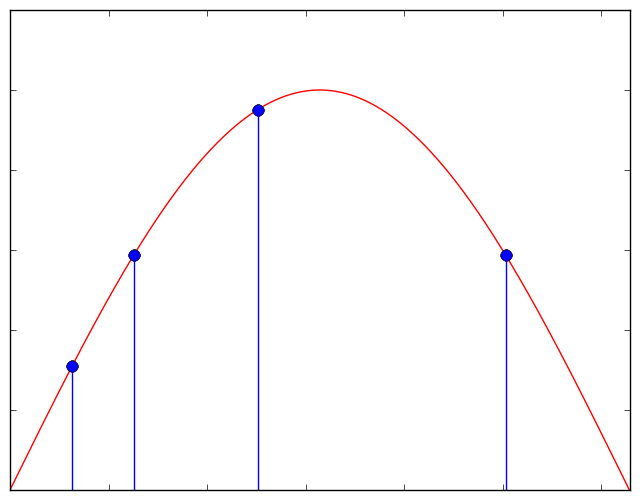
\includegraphics[width=\linewidth]{images/pointbase.png}
      \vspace{-12px}
      \caption{Point based}
      \endminipage
      \hspace{0.025\textwidth}
      \minipage{0.45\textwidth}
      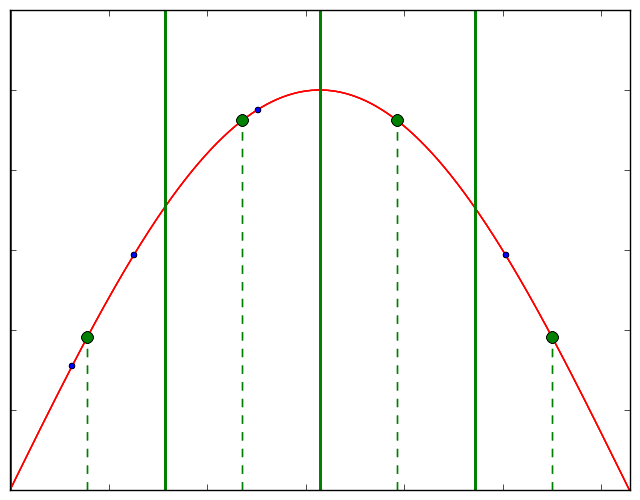
\includegraphics[width=\linewidth]{images/gridbase.png}
      \vspace{-12px}
      \caption{Grid based}
      \endminipage
    \end{figure}
  \end{block}
\end{frame}

\begin{frame}
  \frametitle{Motivation for Sparse Grids}
  \topline
  \vspace{-10px}
  \begin{block}{Suitable for}
    \begin{itemize}
      \item Big datasets
      \item Easily/automatically classifiable data
      \item Medical, seismic, commercial data
    \end{itemize}
  \end{block}
  \begin{block}{Curse of dimensionality}
    \begin{itemize}
    \item The volume of a space is exponential in it's dimensions
    \item The amount of training data required becomes unmanageable
      \begin{itemize}
      \item because of lacking computational/storage capacities
      \item because data aquesition is expensive
      \end{itemize}
    \item Becomes relevant for $d > 3$
    \item \textbf{Applies to full-grid discretization}
    \end{itemize}
  \end{block}
\end{frame}

%%% Local Variables:
%%% TeX-master: "slides"
%%% End: